\documentclass[12pt]{article}
\usepackage[frenchb]{babel} 
\usepackage[T1]{fontenc}
\usepackage[utf8]{inputenc}
%\usepackage{lmodern} 
\usepackage{graphicx}
\usepackage{caption}
\usepackage{multirow}
\usepackage[top=2.5cm, bottom=2.5cm, left=2.5cm , right=2.5cm]{geometry}
%\usepackage{amsmath}
%\usepackage{amsthm}
%\usepackage{amsfonts}
\usepackage{empheq}
\usepackage{setspace}
\usepackage{hyperref}
\hypersetup{pdftitle = {ELE8812 - Rapport de laboratoire}, pdfauthor={Julien Antoine}}
\usepackage{color}
\usepackage{subfigure}
\usepackage{fancyvrb}
\usepackage{SIunits}
\usepackage{numprint}
\usepackage{enumitem}
\usepackage{calc}
\usepackage{listings}
\usepackage{float}
\usepackage{cellspace}
\cellspacetoplimit=4pt
\cellspacebottomlimit=4pt

% ----------------------------------- FANCY HEADER -----------------------------------
\usepackage{fancyhdr}
\pagestyle{fancy}
\renewcommand{\headrulewidth}{0.5pt}
%\fancyhead[C]{\textbf{page \thepage}} 
\fancyhead[L]{}
\fancyhead[R]{Rapport de laboratoire 6}

\renewcommand{\footrulewidth}{0.5pt}
\fancyfoot[C]{\textbf{\thepage}} 
\fancyfoot[L]{Polytechnique Montréal}
\fancyfoot[R]{ELE8812}
% ------------------------------------------------------------------------------------


\providecommand{\e}[1]{\ensuremath{\cdot 10^{#1}}}
\newcommand{\question}{\noindent$\bullet$\;\;}
\newcommand{\eau}{\ensuremath{\text{H}_2 \text{O}}}
\newcommand{\dio}{\ensuremath{\text{CO}_2}}
%\addto\captionsfrancais{\renewcommand{\chaptername}{Labo}}


\hyphenation{HyperLogLog experimental techno-logy according develop-ment}


\begin{document}

\begin{titlepage}
\newcommand{\HRule}{\rule{\linewidth}{0.5mm}} % Defines a new command for the horizontal lines, change thickness here

%-------------------------------------------------------------------------------------
%	LOGO SECTION
%-------------------------------------------------------------------------------------
\centering

\includegraphics[width = 0.33\textwidth]{../../logo}\\[5cm] 
\centering
%-------------------------------------------------------------------------------------
%	TITLE SECTION
%-------------------------------------------------------------------------------------
\HRule \\[0.4cm]
{ \huge \bfseries ELE8812 -- Rapport de laboratoire 6}\\[0.4cm] 
{ \LARGE \bfseries Détection de contours}\\
\HRule \\[1cm]
%-------------------------------------------------------------------------------------
%	AUTHOR SECTION
%-------------------------------------------------------------------------------------
\begin{minipage}{0.45\textwidth}
\begin{center} 
\large
Julien \textsc{Antoine}\\
1813026
\end{center}
\end{minipage}
~
\begin{minipage}{0.45\textwidth}
\begin{center} 
\large
Maxime \textsc{Schmitt}\\
1719088
\end{center}
\end{minipage}\\[8cm]
%-------------------------------------------------------------------------------------
%	DATE SECTION
%-------------------------------------------------------------------------------------
\begin{center}
{\Large 19 avril 2016}
\end{center}
%-------------------------------------------------------------------------------------
\vfill 
\end{titlepage}



\section{Introduction}
Ce dernier travail pratique a pour sujet la détection de contours au sein d'une image. Trois différentes méthodes et leurs paramètres seront analysés: la méthode du gradient, celle de Marr-Hildreth, et celle de Canny.


\section{Méthode du gradient}
La méthode du gradient a la particularité d'être un assemblage de deux détections uni-dimensionnelles, une horizontale et une verticale. Les contours globaux sont obtenus ainsi:
\begin{equation}
	G = \sqrt{G_x^2 + G_y^2}
\end{equation}

\paragraph{}
Les 3 contributions sont observables à la \autoref{fig:sobel}, chacune ayant sa propre colonne. Les lignes permettent quant à elles d'observer l'influence du seuil sur la détection des contours: au milieu le seuil par défaut, en haut un seuil supérieur et en bas inférieur à celui par défaut. On constate ainsi que plus le seuil diminue, plus les contours apparaissent (en vert, superposés à l'image originale), et inversement.


\begin{figure}[!h]
  \centering
  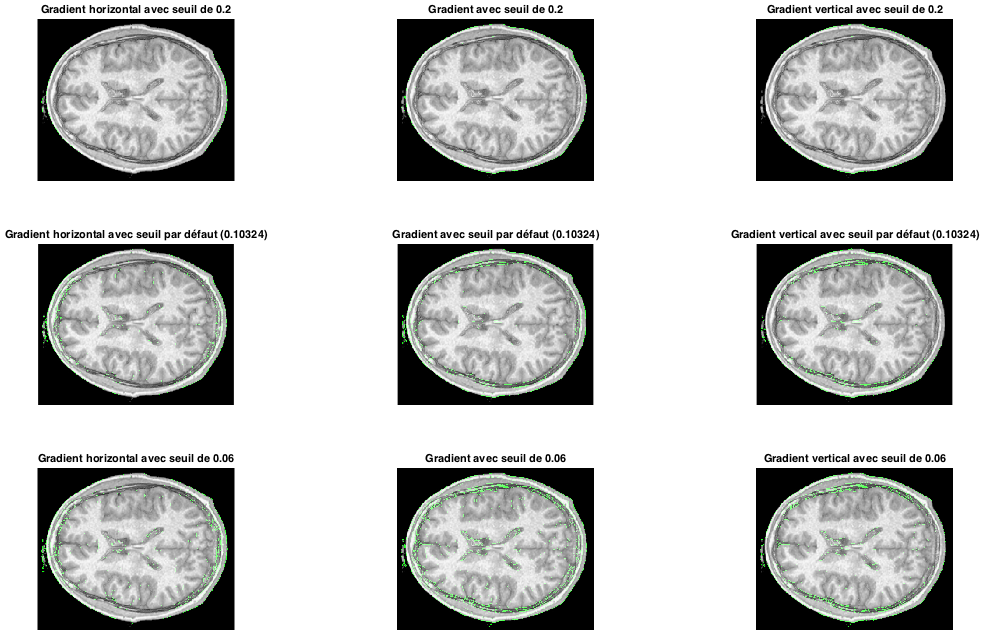
\includegraphics[width = \textwidth]{sobel2}
  \caption{Méthode du gradient et influence du seuil}
  \label{fig:sobel}
\end{figure}



\section{Méthode de Marr-Hildreth}
La méthode de Marr-Hildreth utilise le laplacien de gaussiennes. Deux paramètres influencent le résultat final: le seuil et l'écart-type $\sigma$. La \autoref{fig:marr} représente les résultats obtenus en fonction de ces deux paramètres. La ligne du haut joue sur le seuil, et celle du bas sur l'écart-type de la gaussienne. Dans la colonne centrale apparait l'image originale, dans celle de gauche le paramètre a été diminué, et dans celle de droite il a été augmenté.

\subsection{Influence du seuil}
Comme pour la méthode du gradient, les contours détectés augmentent lorsque le seuil diminue.

\subsection{Influence de l'écart-type}
Les contours sont plus nombreux lorsque l'écart-type diminue. Ceci est normal étant donné que plus l'écart-type est grand, plus la gaussienne va rendre l'image floue et donc les détails vont disparaitre plus fort que pour un petit écart-type. Les contours étant justement représentatifs des détails, aux plus ces derniers sont nombreux, au plus les contours le seront aussi.

\begin{figure}[!h]
  \centering
  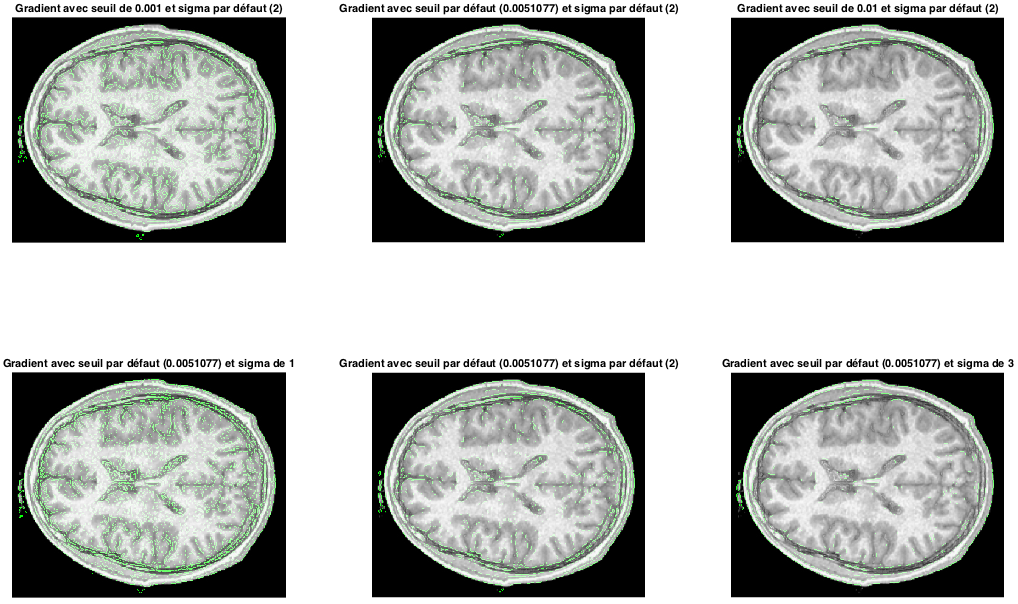
\includegraphics[width = \textwidth]{marr}
  \caption{Méthode de Marr-Hildreth et influence du seuil et de l'écart-type}
  \label{fig:marr}
\end{figure}



\section{Méthode de Canny}
La méthode de Canny est la plus évoluée, elle utilise à la fois deux seuils successifs et un écart-type. Les résultats sont représentés de la même manière que pour Marr-Hildreth à la \autoref{fig:canny}. Contrairement à ce qu'indique la figure, l'écart-type par défaut est $\sqrt{2}$ au lieu de 2. On constate que les résultats sont meilleurs que pour les deux méthodes précédentes, avec des contours mieux définis et plus en accord avec la réalité. L'influence des paramètres est par contre plus compliquée à distinguer sur la figure. On peut cependant remarquer qu'en diminuant le premier seuil et en augmentant le deuxième, moins de contours sont détectés. Dans le cas inverse, on n'observe pas de différence si flagrante, mais un peu plus de contours sont détectés.

\begin{figure}[!h]
  \centering
  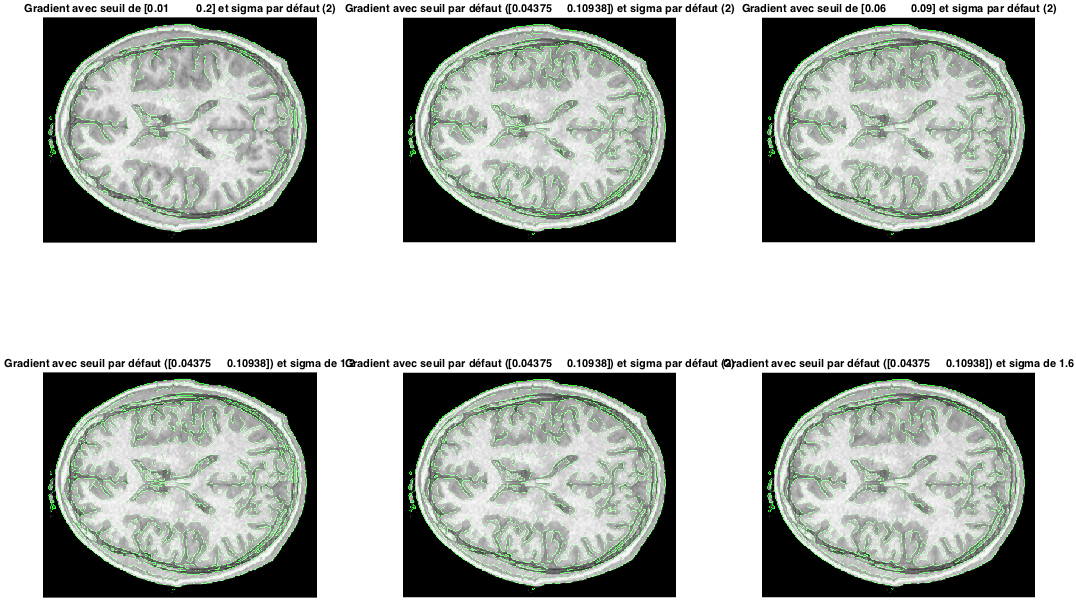
\includegraphics[width = \textwidth]{canny}
  \caption{Méthode de Canny et influence des seuils et de l'écart-type}
  \label{fig:canny}
\end{figure}






\end{document}